\documentclass[paper=a4, fontsize=11pt, BCOR=13mm, DIV=13, headinclude, toc=index, toc=bibliography, english, twoside, parskip]{scrreprt}
% Die verwendete Dokumentenklasse ist scrreprt. Die verwendeten Optionen sind:
%
% paper=a4              Papier ist a4.
% fontsize=11pt         Schrifgröße ist 11.
% DIV=13                Das Papier wird in d viele Spalten und d' viele Zeilen eingeteilt. Die Werte werden aus DIV berechnet.
% BCOR=1cm              Definiert den Patz, der auf der Innenseite beim Binden verloren geht.
% headinclude           sorgt dafür, dass genug Platz für die Header vorhanden ist.
% toc=index             legt im Inhaltsverzeichnis einen Eintrag für das Stichwortverzeichnis an.
% toc=bibliography      legt im Inhaltsverzeichnis einen Eintrag für das Literaturverzeichnis an.
% english               englische Worte wie "Chapter" und "References".
% twoside               Beidseitiges Dokument, wie in einem Buch.


%If you don't want this fancyheaders comment out lines 17 to 24
% Fancyheader
\usepackage{fancyhdr}                   % Wie der Name schon sagt, um fancy Header zu generieren.
\pagestyle{fancy}                       % Fancy Header sollen angezeigt werden
\renewcommand{\sectionmark}[1]{\markright{\thesection.\ #1}{}}    % Verhindert dass rightmark ausschließlich Grußbuchstaben benutzt
\fancyhead[LE,RO]{\rightmark}           % Links bei geraden und rechts bei ungeraden Seitenzahlen soll der Name der Section stehen.
\fancyhead[LO,RE]{}                     % Links bei ungeraden und rechts bei geraden Seitenzahlen soll nichts stehen.
\fancyfoot[C]{}                         % Keine mittigen Seitenzahlen
\fancyfoot[LE,RO]{\thepage}             % Seitenzahlen unten in die jeweilige äußere Ecke





\setcounter{secnumdepth}{3}     % Nummerierungstiefe (chapter, section, subsection, ...).
\setcounter{tocdepth}{3}        % Nummerierungstiefe im Inhaltsverzeichn is.

\usepackage[linesnumbered,ruled,vlined]{algorithm2e}    % Algorithmen setzen.
\newcommand{\SkipBeforeAndAfter}{\vspace{8mm}}
%\SetAlgoSkip{SkipBeforeAndAfter}
%\SetAlgoSkip{bigskip} 
%\usepackage{algorithm}
%\usepackage{algpseudocodex}
%\algrenewcommand\algorithmicrequire{\textbf{Input:}}
%\algrenewcommand\algorithmicensure{\textbf{Output:}}
%\algnewcommand{\LeftComment}[1]{\Statex \(\triangleright\) #1}
\usepackage{amsmath,amssymb,amsthm,amsfonts,amsbsy,latexsym}    % "Notwendige" AMS-Math Pakete.
\usepackage{array}                      % Bessere Tabellen.
\renewcommand{\arraystretch}{1.15}      % Tabellen bekommen ein wenig mehr Platz.
\usepackage{bbm}                        % Dicke 1.
\usepackage[utf8]{inputenc}             % utf8 als Eingabeformat. should be loaded before biblatex
\usepackage[backend=biber, style=alphabetic, giveninits=true]{biblatex}  % Gute Erweiterung zu bibtex, Wird für Referenzen benutzt.
\bibliography{masterthesis_your_name_bibliography}   % Die verwendeten Referenzen (.bib-Datei)
\usepackage[hypcap]{caption}            % Damit Hyperrefs bei der figure-Umgebung auf die Figure zeigt statt auf die Caption.
\captionsetup{font=footnotesize} 
\usepackage{hyperref}
\usepackage{cleveref}
\usepackage{datetime}                   % Um \today einzustellen.
\newdateformat{mydate}{\THEDAY{}th \monthname{} \THEYEAR{}}
\usepackage{diagbox}                    % Diagonale in Tabellen.
\usepackage{enumitem}                   % Zum Ändern der Nummerierungsumgenung 'enumerate'
\setlist[enumerate,1]{label=(\roman*)}  % Aufzählungen sind vom Typ 'Klammer auf; kleine römische Zahl; Klammer zu'
\usepackage[T1]{fontenc}                % Bessere Schrift
\usepackage{ifthen}                     % Zum checken ob Parameter leer sind.
\usepackage{lmodern}                    % Bessere Schrift
\usepackage{listings}                   % Code Listings.
\usepackage{mathtools}                  % Subscript unter Summen behandeln. Der Befehl lautet \mathclap.
\usepackage{makeidx}                    % Stichwortverzeichnis.
\makeindex                              % Stichwortverzeichnis erstellen.
\renewcommand{\indexname}{Index}        % Name des Index definieren.
\usepackage{multirow}                   % In Tabellen mehrere Zeilen zu einer machen.
%\usepackage[parfill]{parskip}
\usepackage{rotating}                   % Um Figures zu drehen.
\usepackage{scrhack}                    % Verbessert die Zusammenarbeit von KOMA mit anderen Paketen (z.B, listing).
\usepackage{stackrel}                   % Symbole übereinander stapeln.
\usepackage[dvipsnames]{xcolor}         % Gefärbter Text und so.
\usepackage{tikz}                       % Graphen und kommutative Diagramme. Muss nach xcolor eingebunden werden.
\usepackage{tikz-cd}                    % Kommutative Diagramme.
\usepackage{transparent}                % Braucht mal manchmal für inkscape bilder.
\usetikzlibrary{patterns}               % Zu malen von schraffierten Flächen.

\graphicspath{{pictures/}}              % Pfad in dem die mit Inkscape erstellen Bilder liegen (relativ zum Hauptverzeichnis).

% Workaround, damit keine unnötigen Leerzeichen entstehen.
\let\oldindexdefn\index
\renewcommand*{\index}[1]{\oldindexdefn{#1}\ignorespaces}
\let\oldlabeldefn\label
\renewcommand*{\label}[1]{\oldlabeldefn{#1}\ignorespaces}

% Workaround, Linebreak nach ldots erlaubt.
\newcommand{\origldots}{}
\let\origldots\ldots
\renewcommand{\ldots}{\allowbreak\origldots}


% Symbolverzeichnis
\usepackage[intoc, english]{nomencl}     % Symbolverzeichnis.
% intoc                 die Symbolliste in das Inhaltsverzeichnis aufnehmen.
% english               englische Worte wie "Seite".
\renewcommand{\nomname}{Symbol Index}   % Definiert die Überschrift des Symbolverzeichnises.
\renewcommand{\nomlabelwidth}{80pt}     % Platz der einem Symbol gegönnt wird.
\newcommand{\symbolindex}[4][]{{\nomenclature[#1]{#2}{#3\ifthenelse{\equal{#4}{}}{}{ -- #4}\nomnorefpage}}\ignorespaces}    % Verbesserte Version von "\nomenclature". Erzeugt Symbol Beschreibung - Referenz.
\renewcommand*{\nompreamble}{\markright{\nomname}}    % Workaround: Fancyhdr schreibt im Symbolverzeichnis sonst den Namen des leztztes Kapitels.
\makenomenclature                       % Symbolverzeichnis erstellen.

% Anklickbare Referenzen (letztes eingebundenes Paket)
\usepackage{hyperref}                   % Referenzen innerhalb des Dokuments anklickbar machen. Achtung: Muss das letzte Paket im Präambel sein.
\hypersetup{                            % Optionen von hyperref Einstellen.
    colorlinks=true,                    % gefärbte Links an Stelle von Boxen.
    linkcolor=black,                     % Farbe interner Links.
    citecolor=black,                     % Farbe von Referenzen.
    urlcolor=black                       % Farbe von Internetlinks.
}

\usepackage{BA_Titelseite}


%Namen des Verfassers der Arbeit
\author{Solveig Tr\"ankner}
%Geburtsdatum des Verfassers
\geburtsdatum{12. März 2002}
%Gebortsort des Verfassers
\geburtsort{Wiesbaden, Hessen}
%Datum der Abgabe der Arbeit
%\date{\today}
\date{21. M\"arz 2025}

%Name des Betreuers
% z.B.: Prof. Dr. Peter Koepke
\betreuer{Betreuer: Prof. Dr. Jochen Garcke}
%Name des Zweitgutachters
\zweitgutachter{Zweitgutachterin: offen}
%Name des Instituts an dem der Betreuer der Arbeit tätig ist.
%z.B.: Mathematisches Institut
%\institut{Institut XYZ}
%\institut{Mathematisches Institut}
%\institut{Institut f\"ur Angewandte Mathematik}
\institut{Institut f\"ur Numerische Simulation}
%\institut{Forschungsinstitut f\"ur Diskrete Mathematik}
%Titel der Bachelorarbeit
\title{Data Visualization with t-SNE in Theory and Practice}
%Do not change!
\ausarbeitungstyp{Bachelorarbeit Mathematik}


%       Theoreme
\theoremstyle{definition}               % Name: dick            Text: normal.
%\newtheorem{defi}{Definition}[section]  % Der Zähler ist defi = Sectionzähler.1 . Sectionzähler soll bei Benutzung von defi nicht erhöht werden.
\newtheorem{defi}{Definition}[chapter]
\newtheorem*{defi*}{Definition}
\newtheorem{example}[defi]{Example}
\newtheorem{notation}[defi]{Notation}
\newtheorem{rem}[defi]{Remark}
\AtBeginEnvironment{rem}{%
  \pushQED{\qed}\renewcommand{\qedsymbol}{$\triangle$}%
}
\AtEndEnvironment{rem}{\popQED\endexample}
\newtheorem{defcor}[defi]{Definition/Corollary}
\newtheorem{defprop}[defi]{Definition/Proposition}
\newtheorem{defthm}[defi]{Definition/Theorem}

\newtheorem*{idea}{Idea}
\newtheorem*{question}{Question}
\newtheorem*{obs}{Observation}
\newtheorem*{prob}{Problem}
\newtheorem*{but}{But}
\newtheorem*{reci}{Recipe}

\theoremstyle{plain}
\newtheorem*{conj}{Conjecture}
\newtheorem{cor}[defi]{Corollary}
\newtheorem{lem}[defi]{Lemma}
\newtheorem{prop}[defi]{Proposition}
\newtheorem*{prop*}{Proposition}
\newtheorem{thm}[defi]{Theorem}
\newtheorem*{thm*}{Theorem}


%       Makros
\newcommand{\bA}{\mathbb{A}}
\newcommand{\bB}{\mathbb{B}}
\newcommand{\bC}{\mathbb{C}}
\newcommand{\bD}{\mathbb{D}}
\newcommand{\bE}{\mathbb{E}}
\newcommand{\bF}{\mathbb{F}}
\newcommand{\bG}{\mathbb{G}}
\newcommand{\bH}{\mathbb{H}}
\newcommand{\bI}{\mathbb{I}}
\newcommand{\bJ}{\mathbb{J}}
\newcommand{\bK}{\mathbb{K}}
\newcommand{\bL}{\mathbb{L}}
\newcommand{\bM}{\mathbb{M}}
\newcommand{\bN}{\mathbb{N}}
\newcommand{\bO}{\mathbb{O}}
\newcommand{\bP}{\mathbb{P}}
\newcommand{\bQ}{\mathbb{Q}}
\newcommand{\bR}{\mathbb{R}}
\newcommand{\bS}{\mathbb{S}}
\newcommand{\bT}{\mathbb{T}}
\newcommand{\bU}{\mathbb{U}}
\newcommand{\bV}{\mathbb{V}}
\newcommand{\bW}{\mathbb{W}}
\newcommand{\bX}{\mathbb{X}}
\newcommand{\bY}{\mathbb{Y}}
\newcommand{\bZ}{\mathbb{Z}}

\newcommand{\bfn}{\mathbf{n}}
\newcommand{\bfx}{\mathbf{x}}
\newcommand{\bfy}{\mathbf{y}}
\newcommand{\bs}[1]{{\boldsymbol#1}}

%\newcommand{\dd}{\mathrm{d}} 
\newcommand{\dd}{\operatorname{d}\!}
\newcommand{\inv}{^{-1}}
\newcommand*{\hm}{^H}
\newcommand*{\tp}{^T}

\newcommand\cconj[1]{\mathop{\overline{#1}}}
\newcommand\closure[1]{\overline{#1}}

\DeclareMathOperator{\spn}{span}
\DeclareMathOperator{\intr}{\text{int}}
\DeclareMathOperator{\rk}{\text{rank}}
\DeclareMathOperator{\diag}{diag}
\DeclareMathOperator{\Ima}{\text{Im}}

%\DeclarePairedDelimiter{\abs}{\lvert}{\rvert}
%\DeclarePairedDelimiter{\norm}{\lVert}{\rVert}

\newcommand\comment[1]{\textcolor{magenta}{\emph{#1}}}


\begin{document}
% Titelseite
\maketitle              % Titelseite ausgeben

\begin{abstract}
    \textbf{Abstract (English)}

    We propose a numerical method to compute stochastic quantities of interest of the Dirichlet Laplacian eigenvalue problem on randomly shaped domains.
    Our approach aims to exploit the stochastic properties of eigenspaces, which, contrary to individual eigenpairs, remain meaningful for eigenvalues of higher multiplicity.
    Using a representation formula, one can obtain an equivalent nonlinear eigenvalue problem for the single layer boundary integral operator, which we discretize by means of a Galerkin boundary element method.
    We employ a contour integral method to solve the discretization by reducing it to a linear eigenvalue problem that inherits its structure. This means that it has the same eigenvalues and multiplicities, and it is possible to obtain approximations of the corresponding eigenfunctions.
    We present a multilevel Monte Carlo quadrature method with a meaningful sampling strategy where we relate the eigenspaces to each other using invariant reference spaces, which allows for a satisfactory computation of expectations of eigenvalues.
    A numerical experiment that validates our proposed approach is given.
    %In this thesis we consider stochastic nonlinear operator-valued eigenvalue problems, in particular the 


    \vspace{2em}
    \textbf{Abstract (German)}

    Wir stellen eine numerische Methode zur Berechnung stochastischer Gr\"{o}\ss en des Dirichlet-Laplaceschen Eigenwertproblems auf zuf\"{a}llig geformten Gebieten vor.
    Unser Ansatz nutzt die stochastischen Eigenschaften der Eigenr\"{a}ume aus, die, im Gegensatz zu den individuellen Eigenpaaren, auch bei vielfachen Eigenwerten bedeutsam bleiben.
    %Im Rahmen der Eigenwertprobleme f\"{u}r holomorphe Fredholm-Operator-wertige Funktionen, kombinieren wir Wissen zur Galerkin-Randelement-Methode für dieses Problem mit einer Kontur-Integral-Methode zur L\"{o}sung nichtlinearer Eigenwertprobleme, um unser Problem auf ein lineares Eigenwertproblem zu reduzieren, das die Struktur des urspr\"{u}nglichen Problems beibehält, das hei\ss t, es hat die gleichen Eigenwerte und Vielfachheiten und es ist möglich, Approximationen der entsprechenden Eigenfunktionen zu erhalten.
    Mithilfe einer Darstellungsformel kann man das Problem äquivalent als ein nichtlineares Eigenwertproblem für den entsprechenden Einfachschichtoperator formulieren. Dieses diskretisieren wir über eine Galerkin-Randelement-Methode.
    Zum Lösen des nichtlinearen Eigenwertproblems verwenden wir eine Kontur-Integral-Methode, die die Diskretisierung auf ein lineares Eigenwertproblem reduziert, das die Struktur des urspr\"{u}nglichen Problems beibehält.
    Das hei\ss t, dass es die gleichen Eigenwerte und Vielfachheiten hat und es möglich ist, Approximationen der entsprechenden Eigenfunktionen zu erhalten.
    Wir stellen eine Multilevel-Monte-Carlo-Simulation vor, um Erwartungswerte der Eigenwerte zu berechnen.
    Dabei verwenden wir eine sinnvolle Sampling-Strategie, bei der wir Eigenräume über gemeinsame Referenzräume miteinander in Verbindung setzen.
    Wir präsentieren numerische Resultate, die unsere Vorgehensweise unterstützen.

\end{abstract}
\cleardoublepage

\setcounter{page}{5}    % Die Titelseite und die darauffolgende leere Seite sollen gefälligst Seite 1 und 2 sein.
\tableofcontents        % Inhaltsverzeichnis ausgeben
%\listofalgorithms

% Einleitung
\cleardoublepage        % Kapitel immer rechts beginnen
\chapter{Introduction}

In our modern world, we are confronted with an ever-growing amount of data. 
Statista estimated the amount of data created, captured, copied and consumed worldwide in 2023 to be a staggering 123 zetabytes, up from two zetabytes in the year 2010 \cite{Statista}.
As the amount of data grows, it also becomes much harder to analyze. 
What makes data analysis even harder is when the dimensionality of the data grows. 
This is increasingly the case in areas such as computer vision, where images are represented by hundreds if not thousands of pixels and natural language processing, where words are transformed into high-dimensional vectors, for example via word2vec \cite{word2vec}.
With such high-dimensional data, it is impossible to just \enquote{quickly take a look at it}. 
Traditional data visualization methods, such as boxplots or standard scatterplots are unable to visualize more than three dimensions effectively. 

\textcolor{red}{A sentence I like from \cite{vdMaa14}: \enquote{Visual exploration is an essential component of data analysis, as it allows for the development of intuitions and hypotheses for the processes that generated the data.}} 

To address this problem, new methods for visualizing high-dimensional data have been proposed. 
The t-Stochastic Neighbour Embedding (t-SNE) algorithm was first developed in 2008 \cite{vdMaa08} and built on prior work on Stochastic Neighbour Embeddings \cite{Hinton02}. 
It has gained a lot of popularity in bioinformatics (cite other biology papers), especially in  single-cell transcriptomics (cite Tasic, macosko, Cao). 
It is also used in cancer research (cite cancer papers here). 
But the use of t-SNE extends to very diverse areas, from finance (cite finance paper here) to computer security and natural language processing. 

\textcolor{red}{maybe mention that t-SNE is not only used for visualization, but can for example also be used as preprocessing before applying a clustering algorithm}

This widespread adoption of the algorithm can be explained by its effectiveness at what it sets out to do. Unlike other dimensionality algorithms, t-SNE was developed with the aim of 2D and 3D visualizations of data in mind. 
By focusing on retaining local structures in the low-dimensional embedding, t-SNE often successfully reveals clusters present in the data. 
Since t-SNE addresses the so-called crowding problem (see below), the embeddings it produces are often visually appealing.  

On a high-level, t-SNE works as follows: from the given points, we calculate a probability distribution that measures pairwise similarities between the data points. 
For the low-dimensional embedding, we start with some data points in 2D or 3D and also construct a distribution of pairwise similarities between these points. 
The t-SNE algorithm then iteratively modifies the location of the low-dimensional datapoints such that the difference between these two distributions, as measured by the Kullback-Leibler divergence, is minimized. 
A different way to understand the algorithm is through the lense of dynamical systems, as described by \cite{LinStei22}. 
One can think of every datapoint as a physical particle which experiences two types of forces: an attractive force to its nearest neighbors in the high-dimensional space and a repulsive force towards all other particles \cite{KoBe19SingleCell}. 

Although t-SNE often works well, there are also some drawbacks to the method. 
Firstly, t-SNE requires the practitioner to make choices regarding the values of some hyperparameters. 
While common libraries \cite{openTSNE, sklearn_api} come with standard parameter settings, it is not uncommon in practice to run the algorithm multiple times with different parameters. 
In particular, the impact of the perplexity parameter, which determines the number of neighbors we consider when constructing the high-dimensional probability distribution, has been studied extensively (\textcolor{red}{include all perplexity citations here}). 

As pointed out by \cite{KoBe19SingleCell}, the perplexity parameter is often perceived as being the only parameter that needs tuning. 
But \enquote{under the hood [...] there are also
various optimisation parameters (such as the learning rate, the
number of iterations, early exaggeration factor, etc.)} \cite{KoBe19SingleCell}, which have been shown to also have a great impact on the quality of the embedding. 
This is problematic, since it is impractical to tune every single parameter and different parameter choices can lead to very different results, making it hard to interpret the results. 
Furthermore, the exact impact of each of these parameters on the embedding is not entirely clear, especially to practioners who are not experts in the field of dimensionality reduction. 


Secondly, there is still a lack of understanding of the internal workings of the algorithm. 
After t-SNE became popular, there also began to appear papers investigating it from a theoretical viewpoint. 
For example, several clustering guarantees have been proposed and the behaviour of t-SNE as the number of datapoints goes to infinity has been studied (\textcolor{red}{add citation here}). 
But difficulties formulating theorems that are applicable to real-world datasets persist, with papers making a number of assumptions that are sometimes disconnected from practice. 

\section*{Objective of This Work}
The goal of this thesis is to provide an overview of the current state of research on both the theoretical and practical aspects of the t-SNE algorithm.  
In particular, we aim to investigate how well the theoretical research on t-SNE carries over to practical applications with real world data. 
We also want to explore the purely practical and algorithmic aspects, with a focus on exploring how t-SNE can be accelerated via automatic stopping \cite{belkina19} and running experiments on hyperparameters that have been not been as extensively studied yet. 
 

\section*{Structure of the Thesis}
We start by giving an overview of dimensionality reduction methods in Chapter 2 before discussion the t-SNE algorithm in detail in Chapter 3. 
In Chapter 4, we present the current state of theoretical research on t-SNE, with a focus on clustering guarantees and behavior in the large-data limit. 
Afterwards, we consider the practical aspects of t-SNE in Chapter 5, including techniques to accelerate the algorithm and hyperparameter optimization. 
Finally, in Chapter 6 we run a range of experiments using different datasets and test various hyperparameter settings. 

\section*{Contributions}
\begin{itemize}
    \item We summarize the existing theoretical literature on t-SNE. 
    \item We give an overview of the current guidelines for choosing parameters. 
    \item We implement the automatic stopping strategy outlined in \cite{belkina19} on top of the state-of-the-art openTSNE library \cite{openTSNE}. 
    \item We test the claims in \cite{murray2024largedatalimitsscaling} empirically for the first time. 
    \item We perform a detailed hyperparameter study on datasets of different sizes. 
\end{itemize}

\section*{Acknowledgements}
I would like to thank Prof. Dr. Garcke for suggesting this interesting topic and guiding me along the way. 
I also want to thank Dr. Bohn for agreeing to be second advisor. I also want to thank the developers of the openTSNE library for having written such a nice library that made everything a lot easier. 
Finally, I want to thank Jimena for proofreading this work. 





% Modelle für den Modulraum
\cleardoublepage        % Kapitel immer rechts beginnen
\chapter{Dimensionality Reduction}\label{chapter:dimensionality-reduction}
This chapter is supposed to provide more context for t-SNE as a nonlinear dimensionality reduction method. 
\begin{itemize}
    \item Many problems exist with high-dimensional data, see (\ref{section:curse}). This is a problem for instance in many ML algorithms, which may suffer from an increased computational cost and decreased performance due to the curse of dimensionality, when the input data has too high of a dimension. 
    \item the goal of dimensionality reduction is to alleviate these issues by mapping high-dim data to a low-dim space whilst preserving as much meaningful structure as possible (don't use this as is)
    \item beyond the realm of data visualization, dimensionality reduction methods are also used for preprocessing before any downstream applications / algorithms. For example, they can improve the performance of clustering algorithms (add reference)
\end{itemize}

\section{The Curse of Dimensionality}\label{section:curse}
The curse of dimensionality, first decribed by \textcolor{red}{[citation here]}, is a broad term, encompassing several phenomena that appear in high dimensions and that make working with high-dimensional data difficult. 

First of all, we should remember that we can never expect a low-dimensional embedding to fully preserve the structure of data with a higher intrinsic dimensionality. Take for example a tetrahedron in the three-dimensional space. It is then impossible to map the tetrahedron to the two-dimensional plane with all distances preserved. 

Also, distances become less meaningful as the dimension increases. (\textcolor{red}{why? explain this more})

Then there is the problem of data sparcity. Consider for instance the tessellation of hypercubes with a Cartesian grid. The number of points needed for this tessellation increases exponentially with the dimension \textcolor{red}{[citation here, book: nonlinear dimensionality reduction techniques]}. 

Finally, and most importantly for t-SNE, there is the crowding problem. 
This simply refers to the fact that there is not enough space to accomodate all neighbors in the lower dimension. 
With an algorithm favoring preservation of local structure, this means that points that are only moderately far from each other have to be placed much further away in the low dimensional map (\textcolor{red}{TODO: maybe insert picture of example here?}). 
This means we have small attractive forces between moderately distant neighbors. 
But even this small number is enough to force all the points to be very close to each other and concentrate in the middle of the map - if we do not have repulsive forces that is. 

\begin{itemize}
    \item different distribution of pairwise distances: volume of a sphere centered on datapoint $x_i$ scales as $r^m$, where $r$ is radius, $m$ is dimension (this is somehow related to the crowding problem) \cite{vdMaa08}
    \item TODO: read up on \enquote{norm concentration} or the \enquote{concentration of measure}
    \item TODO: maybe read WissRech Skript on this section and reference it 
\end{itemize}

\section{Linear and Nonlinear Methods}
One generally distinguishes between linear and nonlinear dimensionality reduction techniques. Another, less clear, differentiation can also be made between techniques that focus on perserving local vs. global structure. 

Some desirable characteristics of dimensionality reduction methods are: reproducibility (no randomness), easy out-of-sample extension, little parameter sensitivity, interpretability.  

Notes from \cite{vdMaa08}: 
\begin{itemize}
    \item there have been various proposals that differ in the type of structure they preserve 
    \item linear techniques: PCA and classical MDS focus on keeping low-dimensional representations of dissimilar datapoints far apart - PCA maximises variance 
    \item often though, high-dimensional data does not lie on a linear space but instead on or near a non-linear (low-dimensional) manifold. here, it is usually more important to keep the low-dimensional representations of very similar datapoints close together. this is something that cannot be done with a linar mapping. 
\end{itemize}

Maybe the most popular linear method is Principal Component Analysis (PCA). It assumes that the data primarily varies along a few directions. It projects the data onto the axes of most variance (and minimizing loss this way). Mathematically, given $X \in \mathbb{R}^{N \times d}$, PCA finds the eigenvectors of the covariance matrix and then orders them by corresponding eigenvalues. A new basis is formed by taking the top $k$ eigenvectors. 
\textcolor{red}{TODO: properly introduce PCA, including algorithm}

Advantages: linear complexity, very interpretably, parametric method makes embedding new points easy. 

A nonlinear method worth mentioning is UMAP. It builds a graph-based representation of the data and optimizes a fuzzy topological structure. Another very popular method is t-SNE, to which the rest of the thesis is devoted. 

\cleardoublepage        % Kapitel immer rechts beginnen
\chapter{t-SNE}\label{chapter:t-sne}

The t-SNE algorithm was first proposed in 2008 by Laurens van der Maaten and Geoffrey Hinton \cite{vdMaa08}. 
This built on previous work by Hinton and Roweis, who proposed the precursor \enquote{Stochastic Neighbor Embedding} algorithm in 2002 \cite{Hinton02}. 

\section{Basic t-SNE Algorithm}
This section closely follows the Theoretical Foundations Paper \cite{JMLR:v23:21-0524} and \cite{vdMaa08} so far. 

Let $\{x_1, \dots , x_n \}$ with $x_i \in \mathbb{R}^d$ for all $1 \leq i \leq n$ be the a set of high-dimensional points we wish to visualize.
We initialize a low-dimensional map $\{y_1, \dots , y_n\} \subset \mathbb{R}^2$ (Sometimes, a three-dimensional map is also considered. For the purpose of this thesis, we stick to two-dimensional maps). 

\subsection{Measuring High-Dimensional Similarities}

Instead of using the raw Euclidean distances between the high-dimensional data points, t-SNE measures pairwise similarities via probabilities. 
We define a joint probability distribution over all pairs of data points $\{(x_i, x_j)\}_{1 \leq i \neq j \leq n}$ via  
\begin{equation}
    p_{j|i} =  \frac{\exp(-\norm{x_i - x_j}_2^2 / 2\sigma_i^2)}{\sum_{k \in \{1,2, \dots, n\} \backslash \{i\}} \exp({-\norm{x_i - x_k}_2^2 / 2 \sigma_i^2})}
\end{equation}
which is then symmetrized to $p_{ij} = \frac{p_{i|j} + p_{j|i}}{2n}$. We set $p_{ii}=0$ for all $i$ since we are only interested in modelling pairwise similarities between points. In matrix form, we write $P = (p_{ij})_{1 \leq i, j \leq n}$. 
Large $p_{ij}$ values indicate that the points $x_i$ and $x_j$ closely resemble each other. 
Intuitively, one can think of $p_{j|i}$ as the probability that $x_i$ would choose $x_j$ as a neighbor if neighbors are chosen according to a Gaussian centered at $x_i$ with bandwidth $\sigma_i$. 

The bandwidths $\sigma_i$ of the Gaussian kernel can be adapted based on a fixed number called perplexity using binary search. See more on this in the section on perplexity. 

One might wonder why it is necessary to symmetrize the similarities. Just taking the $p_{j|i}$ leads to problems for outlier datapoints: since all pairwise distances $\norm{x_i - x_j}^2$ are large for an outlier datapoint $x_i$, all $p_{ij}$ values for this datapoint end up being very small. 
As a result, the location of the low-dimensional map point $y_i$ does not contribute very much to the loss function. With symmetrization, we ensure that $\sum_{j} p_{ij} > \frac{1}{2n}$ for all datapoints $x_i$. 

\subsection{Measuring Low-Dimensional Similarities}
In order to measure similarities between points in the low-dimensional embedding, a first approach would be to also use a Gaussian distribution to convert pairwise distances into probabilities, as above. This is the approach taken originally in SNE \cite{Hinton02}.

However, to address the crowding problem, we instead use the more heavy-tailed Student t-distribution with one degree of freedom (also called a Cauchy distribution). That way, moderate distances in the high-dimensional space will be modeled by much larger distances in the low-dimensional map (since we try to minimize the difference between $p_{ij}$ and $q_{ij}$, see details below). 
\textcolor{red}{\textbf{TO DO}: explain this better}


We then also compute a similarity measure for points in the low-dimensional embedding as follows: 
\begin{equation}
    q_{ij} = \frac{(1+ \norm{y_i - y_j}_2^2)^{-1}}{\sum_{k, l \in \{1,2, \dots, n\}, k \neq l} (1+\norm{y_k - y_l}_2^2)^{-1}}
\end{equation}
where we again define $q_{ii} = 0$ for all $1 \leq i \leq n$. We can collect all of the points in a symmetrical matrix $Q = (q_{ij})_{1 \leq i, j \leq n}$. 


\begin{figure}[h]
    \begin{center}
        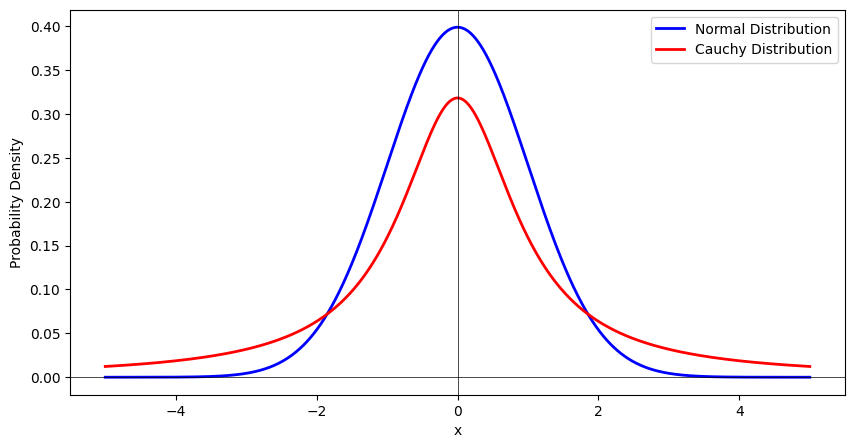
\includegraphics[width=0.9\linewidth]{Gaussian_Cauchy.png}
    \end{center}
\end{figure}

\subsection{The Loss Function}
The goal of the algorithm is now to get the similarities $P$ and $Q$ to be as close to each other as possible. 
A common choice for measuring the distance between two distributions is the Kullback-Leibler divergence. 

\begin{defi}[Kullback-Leibler Divergence]
    The \emph{Kullback-Leibler divergence} between two probability distributions $P$ and $Q$ over the same probability space is defined as:
    \[
    D_{\text{KL}}(P \parallel Q) = \sum_{x \in \mathcal{X}} P(x) \log\frac{P(x)}{Q(x)}
    \]
    for discrete distributions where \(\mathcal{X}\) is the domain of the distributions.
\end{defi}

The t-SNE algorithm now aims to find a low-dimensional representation $\mathcal{Y} = (y_1, \dots, y_n)$ that minimizes the KL-divergence between the similarity matrices $P$ and $Q$. 
We thus define the following loss function: 
\begin{equation}
    C(\mathcal{Y}) = D_{\text{KL}}(P \parallel Q) = \sum_{i,j \in \{1,\dots,n\}, i \neq j} p_{ij} \log \frac{p_{ij}}{q_{ij}}
\end{equation}
which leads to the following optimization problem: 
\begin{equation}
    (y_1, \dots y_n) = \argmin_{y_1, \dots y_n} C(\mathcal{Y}) = \argmin_{y_1, \dots y_n} \sum_{i,j \in \{1,\dots,n\}, i \neq j} p_{ij} \log \frac{p_{ij}}{q_{ij}}.
\end{equation}


Note that the Kullback-Leibler divergence is in fact not a metric, since it is not symmetric. 
One can observe that a large $p_{ij}$ being modeled by a small $q_{ij}$ leads to a bigger summand than using a large $q_{ij}$ to model a small $p_{ij}$. 
This means that our loss function places a large cost on using far-apart points to model points that are close in the original dataset. 
On the other hand, there is only a small cost to model points that are actually far apart as nearby in the embedding. 
This shows that we can expect a bigger focus on the preservation of local structure and is important to keep in mind when interpreting t-SNE embeddings, see \cite{Wa16Distill}. 

\subsection{Gradient Descent to Minimize Loss}
Minimizing the cost function can be achieved using a standard gradient-descent type algorithm, with an updating equation of 
\begin{equation}
    y_i^{(k+1)} = y_i^{(k)} + h \frac{\partial C}{\partial y_i}^{(k)} + m^{(k+1)}(y_i^{(k)} - y_i^{(k-1)}) 
\end{equation}
for $i=1,\dots,n$, where $h >0$ is a prespecified step size parameter, $m^{(k)} > 0$ is a momentum parameter and we denote the gradient of our loss function (with respect to $y_i$) as: 
%\begin{equation}
  %  \frac{\partial C}{\partial y_i}^{(k)} = 4 \sum_{1 \leq j \leq n, j \neq i} (y_j^{(k)} - y_i^{(k)}) S_{ij}^{(k)} \in \mathbb{R}^2 \text{ with } S_{ij}^{(k)} = \frac{p_{ij} - q_{ij}^{(k)}}{1+ \norm{y_i^{(k)}-y_j^{(k)}}_2^2 } \in \mathbb{R}
%\end{equation}
\begin{equation}
    \frac{\partial C}{\partial y_i}^{(k)} = 4 \sum_{1 \leq j \leq n, j \neq i} (p_{ij} - q_{ij}^{(k)}) q_{ij}^{(k)} Z^{(k)} (y_j^{(k)} - y_i^{(k)})
\end{equation}
where $Z$ is a global normalization constant: 
\begin{equation}
    Z^{(k)} = \sum_{m \neq l} (1 + \norm{y_m^{(k)} - y_l^{(k)}})^{-1}. 
\end{equation}
\textcolor{red}{\textbf{TO DO}: Check the gradient here, I'm pretty sure it should be $(y_i - y_j)$ and not the other way around}


% algorithm pseudocode here
\begin{algorithm}[H]
    \caption{Basic version of t-Distributed Stochastic Neighbor Embedding}
    \label{alg:tsne}
    \KwIn{data set $\mathcal{X} = \{x_1, x_2, \dots, x_n\}$, perplexity $\text{Perp}$, number of iterations $T$, learning rate $\eta$, momentum $\alpha(t)$}
    \KwOut{Low-dimensional representation $\mathcal{Y}^{(T)} = \{y_1, y_2, \dots, y_n\}$}


    Compute $p_{ij}$ with perplexity $\text{Perp}$ \;
    Sample initial solution $\mathcal{Y}^{(0)} = \{y_1, y_2, \dots, y_n\} \sim \mathcal{N}(0, 10^{-4} I)$\

    \For{$t = 1$ \KwTo $T$}{
        Compute low-dimensional affinities $q_{ij}$ \;
        Compute gradient $\frac{\delta C}{\delta \mathcal{Y}}$ \;
        Update solution:\;
        \[
        \mathcal{Y}^{(t)} = \mathcal{Y}^{(t-1)} + \eta \frac{\delta C}{\delta \mathcal{Y}} + \alpha(t) (\mathcal{Y}^{(t-1)} - \mathcal{Y}^{(t-2)})
        \]
    }

    \Return $\mathcal{Y}^{(T)}$\
\end{algorithm}
\textcolor{red}{\textbf{TO DO}: make algorithm look nicer}

To optimize the gradient descent prodcedure, \cite{vdMaa08} proposes the following: 
\begin{itemize}
    \item setting the momentum term to $\alpha^{(t)} = 0.5$ for $t<250$ and $\alpha^{(t)} = 0.8$ for $t \geq 250$
    \item set intial learning rate to $\eta = 100$ and update after every iteration adaptively using the adaptive learning rate scheme described by Jacobs \cite{Jacobs1988}
\end{itemize}



\section{Initialization}
here talk about pca init vs random one 
...
\section{Perplexity}
Let us come back to the variance $\sigma_i$ of the Gaussian centered at each datapoint $x_i$. What is a good value to choose? 
If we fixed a single value $\sigma$ to be the same for every datapoint, this is likely not a good choice, because real-life data often does not have a constant density everywhere but instead has sparser and denser regions. 
Given that we want to consider approximately the same number of nearest neighbors for each $x_i$, we opt to choose larger values of $\sigma_i$ for sparse regions and smaller bandwidths for dense regions. 

\textcolor{red}{\textbf{TO DO}: find a better way to describe what perplexity actually does, the following is just taken directly from \cite{vdMaa08}}

Any particular value of $\sigma_i$ induces a probability distribution $P_i$ over all other datapoints. 
The entropy of this distribution increases as $\sigma_i$ increases. 
The user can specify a specific so-called perplexity
\begin{equation}
    \kappa = \text{Perp}(P_i) = 2^{H(P_i)} 
\end{equation}
where $H(P_i) = -\sum_{j} p_{ij} \log_2 p_{ij}$ denotes the Shannon entropy of $P_i$. 

\textcolor{red}{\textbf{TO DO}: do we use $p_{ij}$ or $p_{j|i}$ in the definition of perplexity?}

Then, t-SNE performs a binary search for the value of $\sigma_i$ that produces the user-specified perplexity. 

One can think of perplexity as a smooth measure of the effective \textcolor{red}{\textbf{TO DO}: what does this actually mean?} number of neighbors being considered in the calculation of the $p_{ij}$. As such, larger perplexity values are computationally more expensive. 

\cleardoublepage        % Kapitel immer rechts beginnen
\chapter{Multilevel quadrature of eigenspaces}\label{chapter:multilevel-quadrature}

%\comment{Do I want to restrict myself to this or do I want to take nonlinear eigenvalue problems that depend on a random paramenter in general?}
Now, we recall the original problem (\ref{eq:og-prob}).
We assume that the domain $D(\bs{y})$ is given as a random deformation of a reference Lipschitz domain $D_{\text{ref}}\subset \bR^3$ with piecewise smooth surface $S_{\text{ref}} \coloneq \partial D_{\text{ref}}$.
Further, we assume that this deformation can be encoded in a parameter $\bs{y} \in [-1,1]^{\bN}$ (cf. \cite{DOLZ2022114242}).
We will approximate the parameter space $[-1,1]^{\bN}$ by a finite dimensional space $[-1,1]^N$ where $N$ is large enough.
Our aim is to compute stochastic quantities of interest of the eigenpairs, namely their expectation.
As our parameter space is high dimensional, we want to use a quasi-Monte Carlo method, which is preferred to Monte Carlo due to the higher convergence rate.

When employing sampling-based numerical methods to calculate the expectation, such as quasi-Monte Carlo, the challenge of relating eigenvalues to each other across the samples arises.
Even if the trajectories of the eigenvalues are given by continuously differentiable paths, it is not evident how to track these over the discrete samples, especially when the random parameter is high dimensional, as crossings and bifurcations could occur.
We use an approach that exploits the more meaningful stochastic properties of the eigenspaces \cite{Doelz_Ebert_2024}.

Our goal is to compute the expectations of the eigenvalues that lie within a given contour $\Gamma \subset \bC$.
In order for the method to work, we require that the eigenvalues that lie inside of $\Gamma$ are separated by our contour over the entire parameter space from the rest of the eigenvalues (cf. \cite{kato_perturbation,grubivsic2023stochastic}).

%\section{Modelling of random domains and surfaces}

%%CHANGE OMEGA 
In what follows, let $D_{\text{ref}} \subset \bR^3$ denote a Lipschitz domain with piecewise smooth surface $S_{\text{ref}} \coloneq \partial D_{\text{ref}}$ and $(\Omega, \mathcal{F}, \bP)$ be a complete probability space.
We assume the uncertainty in the obstacle to be encoded by a random domain field \comment{meter cita}.
Hence, we assume the existence of a uniform $\mathcal{C}^1$-diffeomorphism $\mathbf{\chi}_D \colon \closure{D}_{\text{ref}} \times \Omega \to \bR^3$, i.e.
\[
    \lVert \mathbf{\chi}_D (\omega)\rVert _{\mathcal{C}^1(\closure{D}_{\text{ref}};\bR^3)}, \lVert \mathbf{\chi}_D\inv (\omega)\rVert _{\mathcal{C}^1(\closure{D(\omega)};\bR^3)} \leq C  \quad \text{for } \bP\text{-a.e. } \omega \in \Omega
\]
such that
\[
    D(\omega) = \mathbf{\chi}_D (D_{\text{ref}}, \omega).
\]

meter más de lo de cómo pasar al parameter $y\in [-1,1]^N$.
\section{Single-level Monte Carlo quadrature}
We introduce our method first for the single-level case.
Consider nonlinear eigenvalue problems as in \Cref{chapter:cim} now for a parametrized family of functions $T_{\bs{y}} \in H(\Omega, \bC^{m \times m})$ for $\bs{y}\in [-1,1]^{\bN}$, where we take $T_\mathbf{0}$ as the reference element.
Let $k$ be the number of eigenvalues, including multiplicities, inside of the contour $\Gamma$.
We write $A_{\bs{y}, 0}$ and $A_{\bs{y}, 1}$ if \cref{eq:A0,eq:A1} are computed for $T_{\bs{y}}$, respectively.

%For each sample $\bfy \in [-1,1]$, we want to find a suitable quantity to compute for which a meaningful expectation can be found.
We recall \Cref{section:reduction-cim}, where the method to solve nonlinear eigenvalue problems was presented.
After calculating the matrices $A_{\bs{y}, 0}$ and $A_{\bs{y}, 1}$, we computed the eigenvalue decomposition 
\begin{equation}
    \label{eq:svd-A0-param}
    A_{\bs{y}, 0} = V_{\bs{y},0} \Sigma_{\bs{y},0} W_{\bs{y}, 0}\hm.
\end{equation}
%\comment{pensar si quiero resumir aquí brevemente la herleitung, bzw. poner tipo la fórmula de B y de S}.
Now, the central idea of the method is to fix two orthogonal matrices $V_0 \in \bC^{m\times k}$ and $W_0 \in \bC^{l\times k}$, which will replace $V_{\bs{y},0}$ and $W_{\bs{y}, 0}$.
Instead of the singular value decomposition \eqref{eq:svd-A0-param}, we then take
\begin{equation}
    A_{\bs{y}, 0} = V_0 \Sigma_{\bs{y},0} W_0\hm,
\end{equation}
where $\Sigma_{\bs{y},0} = V_0\hm A_{\bs{y}, 0} W_0$ is not necessarily a diagonal matrix anymore.
We see that we can still perform each step of the reduction with this modified decomposition, as the only property needed of $V_{\bs{y},0}$ was that it be orthogonal, so we get
\[ 
    B_{\bs{y}} = V_0\hm A_{\bs{y},1} W_0 \Sigma_{\bs{y},0}\inv = S_{\bs{y}}\Lambda_{\bs{y}} S_{\bs{y}}\inv = V_0\hm V_{\bs{y}} \Lambda_{\bs{y}} (V_0\hm V_{\bs{y}})\inv.
\]
%\comment{y poner aquí las fórmulas de B y S otra vez pero con el $V_0$ fijado}
So, essentially, the major modification is that the matrix of eigenvectors of $B$ is given by $S_{\bs{y}} = V_0\hm V_{\bs{y}}$ instead of $S_{\bs{y}} = V_{\bs{y},0}\hm V_{\bs{y}}$, which means that we are always relating the matrix of eigenvectors of $T_{\bs{y}}$ that is given by $V_{\bs{y}}$ to the same orthogonal matrix $V_0$ instead of taking a different one for each sample.
%\comment{revisar/mejorar esto de qué es la idea}
Then, we compute the expectation of the matrix $B$, which has the same eigenvalues including multiplicities as our original problem, and from which we can directly derive eigenvectors for our original problem, see \Cref{thm:equiv-B-T(z)}.
We summarize the method in \Cref{alg:single-level}.
%\comment{add better explanation of why we do this, why this is a suitable größe}

Let $l \geq k$.
\begin{algorithm}
    \DontPrintSemicolon

    \SetKwInput{Input}{Input}
    \SetKwInput{Output}{Output}
    \SetKw{KwGoTo}{go to}

    \Input{A family $T_{\bs{y}} \in H(\Omega, \bC^{m \times m})$ of parametrized matrices and a contour $\Gamma \subset \Omega$}
    %\Output{An approximation of $\bE[B]$, where $B$... (retains eigenvalues and mulitplicity o así)}
    \Output{An approximation of $\bE[B]$}
    \BlankLine
    Draw a random matrix $\widehat{V} \in \bC^{m\times l}$\;
    Choose two orthogonal matrices $V_0$ and $W_0$ (e.g. using the SVD of $A_{\mathbf{0},0})$\;
    \For{$i = 1,\ldots,M$}{
        Draw a random sample $\bs{y}_i \sim \text{Unif}([-1,1]^N)$\;\label{line:monte-carlo-y}
        Compute $A_{\bs{y}_i, 0}$ and $A_{\bs{y}_i, 1}$\;
        Set $\Sigma_{\bs{y}_i,0} = V_0 A_{\bs{y}_i,0} W_0\hm$\;
        Set $B_{\bs{y}_i} = V_0\hm A_{\bs{y}_i,1} W_0 \Sigma_{\bs{y}_i,0}\inv$\;
    }
    \Return{$B = \frac{1}{M} \sum_{i=1}^M B_{\bs{y}_i}$}
    \caption{Single-level Monte Carlo quadrature for nonlinear eigenvalue problems}\label{alg:single-level}
\end{algorithm}
\begin{rem}
    (a) As $V_0$ and $W_0$ are not the matrices associated to the eigenvalue decomposition of $A_{\bfy_i, 0}$, the matrix $\Sigma_{\bfy_i, 0}$ is not necessarily diagonal anymore.
    Therefore, one should not invert the matrix directly.
    Instead, it is possible to compute $(W_0 \Sigma_{\bfy_i,0}\inv)\tp$ as the solution $X\tp$ of the system of linear equations $\Sigma_{\bfy_i,0}\tp X\tp = W_0\tp$.

    (b) In the current form, the algorithm performs a Monte Carlo quadrature (see \Cref{line:monte-carlo-y}).
    It is also possible to replace it by a quasi-Monte Carlo method. %\comment{igual meto directamente la quasi Monte Carlo methode en el algoritmo, pero entonces sería un poco más unübersichtlich}
\end{rem}
\section{Multilevel Monte Carlo quadrature}
For a more efficient calculation of the quantities of interest, it is also possible to use a multilevel quadrature method \cite{DOLZ2022114242,Giles_2015}.
The main computational effort when considering a stochastic Dirichlet Laplacian eigenvalue problem lies in computing the approximation $\underline{V}(\kappa)$ of the single layer boundary integral operator.
The idea of multilevel Monte Carlo is to perform most simulations with low accuracy at a corresponding low cost and rather few simulations at high accuracy and high cost.
In our case, low accuracy corresponds with using a Galerkin approximation space on a coarser refinement level and accordingly, high accuracy is achieved when using an approximation space with a higher refinement.

Using a multilevel quadrature approach, we obtain
\begin{equation}
    \label{eq:B-multilevel}
    \bE[B] \approx \mathcal{Q}_L^{\text{ML}} [B] = \sum_{\ell=0}^L \mathcal{Q}_{L-\ell} [B^{(\ell)}-B^{(\ell-1)}],
\end{equation}
where $\mathcal{Q}_{\ell}$ is a quadrature rule on level $\ell$.
The approximation $B^{(\ell)}$ is computed using the Galerkin approximation $\underline{V}^{(\ell)}(\kappa)$ of the single layer boundary integral operator of the Helmholtz equation on refinement level $\ell$, setting $B^{(-1)} = 0$. For the approximation error of the multilevel quadrature, it holds a sparse tensor product-like error estimate.
\iffalse
If $\varepsilon_{\ell} \to 0$ is a monotonically decreasing sequence with $\varepsilon_{\ell} \cdot \varepsilon_{L-\ell} = \varepsilon_L$ for every $L\in \bN$ and
\[
    \lVert \mathcal{B}_{L-\ell}-\bE[B]\rVert \leq c_1\varepsilon_{L-\ell} \quad \text{and}\quad \lVert B^{(\ell)}-B\rVert \leq c_2\varepsilon_{\ell}
\]
for some suitable norms and constants $c_1,c_2 > 0$, then
\[
    \lVert \mathcal{Q}_L^{\text{ML}}[B] - \bE[B] \rVert \leq C\varepsilon_L
\]
for a constant $C>0$, \comment{what conditions do we need?}. %given that $B$ is sufficiently regular \comment{revisar esto, tipo cuáles son las condiciones}.
\fi

%\comment{igual conviene otra letra que ml es también la mulitplicity}
Since the size of $\underline{V}^{(\ell)}(\kappa) \in \bC^{m_{\ell} \times m_{\ell}}$ depends on the refinement level, we cannot choose the orthogonal matrices $V_0$ and $W_0$ independent of the level, but need matrices $W_0^{(\ell)}$ and $V_0^{(\ell)}$.
%In particular, this means that the eigenspaces that we fix are not the same across all levels.
If, on a single level, we choose $V_0$ and $W_0$ using the SVD of $A_{\mathbf{0},0} = V_0 \Sigma_0 W_0\hm$, $W_0$ and $V_0$ depend only on $\underline{V}^{(\ell)}(\kappa)$ and $\widehat{V}$.
As we cannot control $\underline{V}(\kappa)$, we consider $\widehat{V}$ instead.

For the contour integral method, the only property required of $\widehat{V}$ is that it has full rank.
Furthermore, for the computation of $A_{\mathbf{0},0}$ and $A_{\mathbf{0},1}$, we are computing $\underline{V}(\kappa)\inv \widehat{V}$.
Since $\underline{V}(\kappa)$ is the system matrix of a Galerkin method, we can interpret $\widehat{V}$ as a matrix of discretized linear forms.
So, instead of choosing the columns of $\widehat{V}$ randomly, we can choose the linear forms randomly in a suitable sense such that $\widehat{V}$ has full rank independently of the ansatz space.
Once we obtain $\widehat{V}^{(\ell)}$ in this fashion, we can compute $V_0^{(\ell)}$ and $W_0^{(\ell)}$ on each level as before.

Regarding the choice of the linear forms, we propose the following.
For each column of $\widehat{V}$, we take a suitable random function that we test against the corresponding ansatz space with the $L^2$-scalar product to get discretized linear forms for each level.
A way of finding appropiate random functions is to choose functions $f(\bfx) = e^{-\frac{\norm{\bfx - \bfm}_2}{\sigma}}$, where $\bfm \in \bR^3, \sigma >0$ are random parameters.

\Cref{alg:multilevel} shows an example of how a multilevel approach for our problem could be implemented.
%\comment{ask about inputs/outputs, what exactly to say there, do I want to take $T$ there or $\underline{V_{\kappa}}$}

Let $l' \geq k$.
\begin{algorithm}
    \DontPrintSemicolon

    \SetKwInput{Input}{Input}
    \SetKwInput{Output}{Output}
    \SetKw{KwGoTo}{go to}

    \Input{Aproximations $T_{\bs{y}}^{(\ell)} \in H(\Omega, \bC^{m \times m})$ of a family of parametrized functions for $\ell = 0,\ldots,L$ and a contour $\Gamma \subset \Omega$}
    \Output{A multilevel approximation $\mathcal{Q}_L^{\text{ML}}[B]\approx \bE[B]$}%, where $B$... (retains eigenvalues and multiplicity o así)}
    \BlankLine
    Generate $l'$ random functions $f_j(\bfx) = e^{-\frac{\norm{\bfx - \bfm_j}_2}{\sigma_j}}, \space j=1,\ldots,l'$, where $m_j \sim \text{Unif}([0,1]^3),\space \sigma_j \sim \text{Unif}([0,1])$\;
    \For{$\ell = 0,\ldots,L$}{
        Compute $\widehat{V}^{(\ell)}$ with columns given by the discretization of the functions $f_j, \space j=1,\ldots,l'$ on the Ansatz space for refinement level $\ell$\;
        Compute the SVD of the matrix $A_{\mathbf{0},0}^{(\ell)} = V_0^{(\ell)H} \Sigma_0^{(\ell)} W_0^{(\ell)}$\;
        \For{$i=1,\ldots, M^{(\ell)}$}{
            Draw a random sample $\bs{y}_i \sim \text{Unif}([-1,1]^N)$\;
            Compute $B_{\bs{y}_i}^{(\ell)}$ and $B_{\bs{y}_i}^{(\ell-1)}$ using $V_0^{(\ell)}$ and $W_0^{(\ell)}$, and $V_0^{(\ell-1)}$ and $W_0^{(\ell-1)}$, respectively\;
            Set $D_{\bs{y}_i}^{(\ell)} = B_{\bs{y}_i}^{(\ell)} - B_{\bs{y}_i}^{(\ell-1)}$\;
            %Compute $A_{\bs{y}_i, 0}^{(\ell)}$ and $A_{\bs{y}_i, 1}^{(\ell)}$\;
            %Set $\Sigma_{\bs{y}_i,0} = V_0 A_{\bs{y}_i,0} W_0\hm$\;
            %Set $B_{\bs{y}_i} = V_0\hm A_{\bs{y}_i,1} W_0 \Sigma_{\bs{y}_i,0}\inv$
        }
        Set $D^{(\ell)} = \frac{1}{M^{(\ell)}} \sum_{i=1}^{M^{(\ell)}} D_{\bs{y}_i}^{(\ell)}$\;
    }
    \Return{$B^{\text{ML}} = \sum_{\ell=1}^L D^{(\ell)}$}
    \caption{Multilevel Monte Carlo quadrature for the Dirichlet Laplacian eigenvalue problem}\label{alg:multilevel}
\end{algorithm}

%\comment{think if i want to include remarks}

\cleardoublepage        % Kapitel immer rechts beginnen
\chapter{Numerical results}\label{chapter:numerical-results}
In this chapter we present a numerical example to showcase the ideas introduced earlier.
As the reference domain, we consider the three-dimensional unit cube $D_{\text{ref}} = (0,1)^3$.
The eigenvalues of \eqref{eq:og-prob} on the reference domain are given by 
\[
    \lambda_k = \pi^2(k_1^2+k_2^2+k_3^2)
\]
with associated eigenfunctions
\[
    u_k(x) = \sin(\pi k_1 x_1)\sin(\pi k_2 x_2)\sin(\pi k_3 x_3)
\]
for all $k = (k_1,k_2,k_3)\in \bN^3$.

For modeling the domain and computing the solution of (\ref{eq:og-prob}), we employ the \texttt{C++} library \texttt{bembel} \cite{Bembel2020}.
We want to find mean values for the eigenvalues $\lambda_k$ where $\kappa_k = \sqrt{\lambda_{k}}$ is located inside of the ellipse with center $\mu = \frac{(\sqrt{3}+\sqrt{6})\pi}{2}$, width $2a = 4$ and height $2b = 0.4$.
The ellipse can be parametrized by $\varphi(t) = \mu + \frac{a+b}{2}e^{it} + \frac{a-b}{2}e^{-it}$ for $t\in [0,2\pi]$.
In the reference case, the contour contains $\kappa_{(1,1,1)} = \sqrt{3}\pi, \kappa_{(1,1,2)} = \kappa_{(1,2,1)} = \kappa_{(2,1,1)} = \sqrt{6}\pi$.
In order to ensure that the eigenvalues stay separated by our contour over the entire parameter space, we scale it by $\alpha = \frac{1}{3}$, i.e. we only take random parameters $\boldsymbol{y} \in [-\frac{1}{3},\frac{1}{3}]^\bN$ instead of  $\boldsymbol{y} \in [-1,1]^\bN$. In practice, we approximate this by $\boldsymbol{y} \in [-\frac{1}{3},\frac{1}{3}]^N$ with $N$ large enough.
\begin{figure}
    \centering
    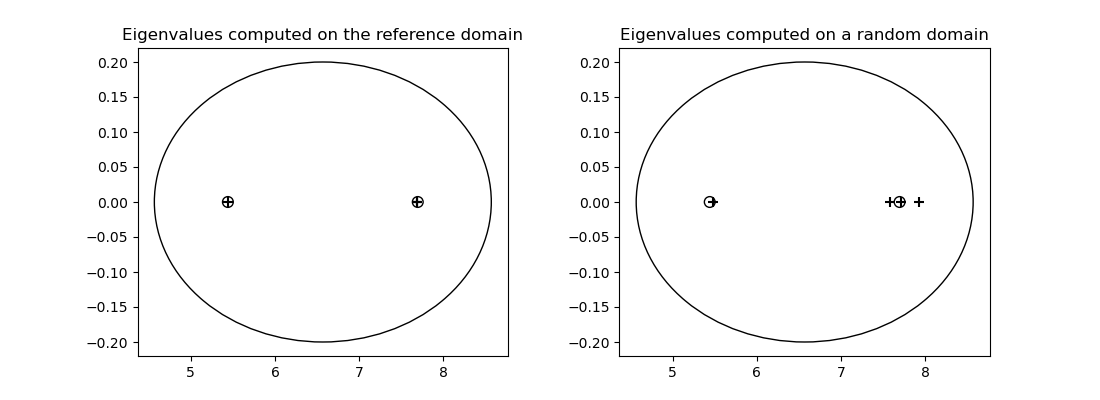
\includegraphics[width=\textwidth]{chapter_numerical_results/both_new_ratio_new_size.png}
    \caption{Two realizations of the contour integral method for a Galerkin approximation (polynomial degree zero and refinement level three) of the single layer boundary integral operator. The open circles indicate the exact eigenvalues on the reference domain, the crosses the approximations computed by the contour integral method.}
    \label{fig:cim}
\end{figure}
\Cref{fig:cim} contains two results of the contour integral method, one on the reference domain and one on a random perturbation of the domain. They show that indeed a bifurcation occurs, as on the reference domain we have an eigenvalue with multiplicity three, while for the random domain we find four different simple eigenvalues.

As we are integrating over a high-dimensional parameter space, we use a multilevel quasi-Monte Carlo quadrature (QMC) with the Kronecker sequence \cite{Dick_Kuo_Sloan_2013}.
Due to the asymptotic convergence rate of $h^{2p+3}$ of the boundary element method for the approximation of the eigenvalues, the number of samples for the quadrature has to be adapted for each level according to $\sim h^{-2p-3}$.
This yields the number of quadrature points as shown in \Cref{tab:number-of-samples}.

\begin{table}[htb]
    \centering
\begin{tabular}{c c c c c}
    \hline
     & $\ell=2$ & $\ell=3$ & $\ell=4$ & $\ell = 5$ \\\hline
    $p = 0$ & 5\,120 & 640 & 80 & 10 \\\hline
    $p = 1$ & 10\,240 & 320 & 10 &  \\\hline
    \end{tabular}
    \medskip
    \caption{Number of samples on the different levels for QMC.}
    \label{tab:number-of-samples}
\end{table}

In order to measure the approximation errors, we compute a reference solution on the finest level for each polynomial degree using a quasi-Monte Carlo method with the Halton sequence \cite{Dick_Kuo_Sloan_2013}.
The error is given in terms of the $\ell^{\infty}$-norm calculated with respect to the eigenvalues, that is, we take the error to be $\max_{i=1,\ldots,k} \abs{\lambda_i^{L} - \lambda_i^{\text{ref}}}$, where $\lambda_1^{L},\ldots,\lambda_k^{L}$ are the eigenvalues of the approximation $\mathcal{Q}_L^{\text{ML}} [B]$ and $\lambda_1^{\text{ref}},\ldots,\lambda_k^{\text{ref}}$ are the eigenvalues of our reference solution for $\bE[B]$.

\begin{figure}
    \centering
    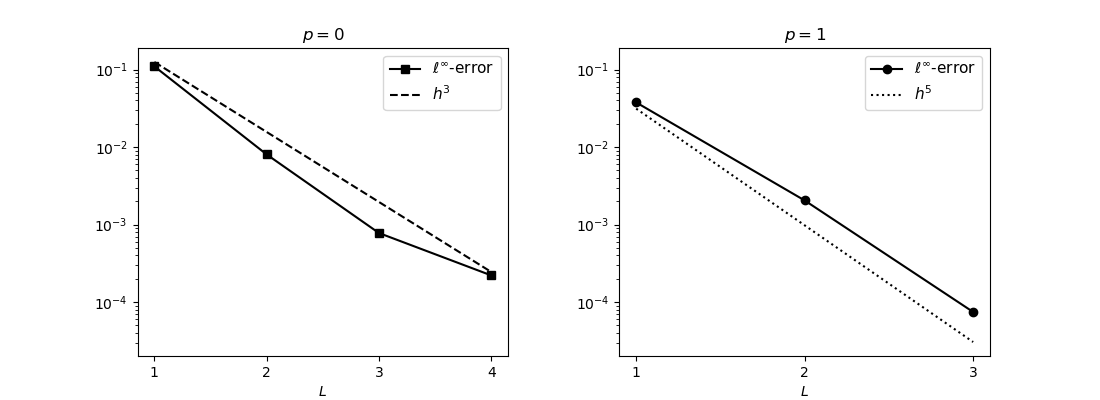
\includegraphics[width=\textwidth]{chapter_numerical_results/plots_new_ratio.png}
    \caption{Convergence of multilevel QMC for the expectation of the eigenvalues. \textit{Left}: Using a BEM with piecewise constant functions. \textit{Right}: Using a BEM with piecewise linear functions.}
    \label{fig:plots}
\end{figure}
\Cref{fig:plots} illustrates the results obtained, where the dashed lines indicate the expected convergence rate of the boundary element method.
We see that the results seem to confirm the theoretical error estimates.
The bend in the error plot where we used piecewise constant approximation spaces could be ascribed to lacking accuracy of our reference solution.
Alas, due to the large number of samples and the high computational cost of evaluating the single layer boundary integral operator, more approximations as well as a better reference solution are out of reach with the available resources.

\cleardoublepage        % Kapitel immer rechts beginnen
\chapter{Conclusions}\label{chapter:conclusions}
The goal of this work was to find a method to compute stochastic quantities of Dirichlet Laplacian eigenvalue problems.
We proposed an approach based on computing expectations of eigenspaces rather than of the individual eigenpairs themselves, which means that we completely avoid the matching problem that arises for the latter quantities.
For this purpose, we required discretization methods to solve the Dirichlet Laplacian eigenvalue problem which retain the structure of the problem.
We have seen that this is the case for the Galerkin approximation of the single layer boundary integral operator as well as for the contour integral method.
Moreover, the contour integral method was a particularly suitable method to solve the nonlinear eigenvalue problem arising from the Galerkin discretization as it allows for a simultaneous computation of various eigenvalues and their eigenspaces.

Our numerical experiments seem to confirm the theoretical results.
So, we have found that we can satisfactorily evaluate stochastic properties of our eigenvalue problem given that we can locate and separate the eigenvalues of interest in and by a contour.
Employing a multilevel quadrature accelerates our method.
Still, the most expensive part of the algorithm, which is markedly computing the approximation of the single layer boundary integral operator, prevents us from computing reference solutions with more samples.

%\cleardoublepage
%\appendix
\chapter*{Appendix}
\addcontentsline{toc}{chapter}{Appendix}
\renewcommand{\thesection}{\Alph{section}}
\section{a}
\section{b}

% Weitere Symbole für das Symbolverzeichnis
\symbolindex[f]{$F$}{A topological or Riemann surface.}{}

% Symbolverzeichnis
\cleardoublepage        % Auch diese sollen auf der rechten Seite beginnen
\printnomenclature      % Symbolverzeichnis ausgeben

% Stichwortverzeichnis
\cleardoublepage        % Auch diese sollen auf der rechten Seite beginnen
\printindex             % Stichwortverzeichnis ausgeben

% Referenzen
\nocite{*}              % Alle Einträge der Bib-Datei sollen in die Referenzen
\cleardoublepage        % Auch diese sollen auf der rechten Seite beginnen
\printbibliography      % Bibliographie ausgeben.

\end{document}